\documentclass{easychair}

\usepackage[utf8]{inputenc}
\usepackage[T1]{fontenc}
\usepackage{amsmath,amssymb,amsfonts}
\usepackage{graphicx}
\usepackage{booktabs}
\usepackage{listings}
\usepackage{xcolor}
\usepackage{enumitem}

\graphicspath{{resources/}}
\setlist{itemsep=1pt,topsep=3pt}

\lstset{
  basicstyle=\ttfamily\small,
  columns=fullflexible,
  keepspaces=true,
  showstringspaces=false,
  breaklines=true,
  xleftmargin=4mm,
  literate=
    {→}{{$\rightarrow$}}1 {∀}{{$\forall$}}1 {∃}{{$\exists$}}1 {∈}{{$\in$}}1
    {ℕ}{{$\mathbb{N}$}}1 {∣}{{$\mid$}}1 {∨}{{$\vee$}}1 {∧}{{$\wedge$}}1
    {≠}{{$\neq$}}1 {≤}{{$\leq$}}1 {⟨}{{$\langle$}}1 {⟩}{{$\rangle$}}1
    {↔}{{$\leftrightarrow$}}1 {λ}{{$\lambda$}}1 {·}{{$\cdot$}}1 {¬}{{$\neg$}}1
    {ü}{{\"u}}1 {ä}{{\"a}}1 {ö}{{\"o}}1 {é}{{\'e}}1
}

\newcommand{\ttt}[1]{\texttt{#1}}
\newcommand{\reading}[1]{\begin{quote}\small #1\end{quote}}

\title{Informalizing Lean}
\titlerunning{Informalizing Lean}

\author{
  Aarne Ranta\inst{1}
  \and
  Claude\inst{2}
}

\institute{
  Department of Computer Science and Engineering,
  Chalmers University of Technology and University of Gothenburg, Sweden\\
  \email{aarne.ranta@cse.gu.se}
  \and
  Claude Code, an AI coding agent by Anthropic, working in the first author's checkout
}

\authorrunning{Ranta and Claude}

\begin{document}

\maketitle

\begin{abstract}
Lean and its library Mathlib contain a large and growing part of mathematics in machine-checked
form, but the formal code is hard to read for anyone who is not a Lean expert, and the code
produced by autoformalization is read by even fewer. We describe a system that translates Lean
declarations, with their statements, definitions and proofs, into ordinary mathematical
language in five natural languages. The translation goes through the logical framework
Dedukti and the Informath grammar, written in Grammatical Framework (GF), and is symbolic: it is
compositional and does not invent content. The main bottleneck is the symbol table, which tells
how each Lean constant is to be worded. We infer it for all of Mathlib's definitions from
their docstrings and names, checking each candidate with the grammar and replacing the words
that it lacks by words of its lexicon: 69\% of 38,667 definitions get a wording. All of them are
then read in English, as formulas and in French, with their definientia: 99\% get a reading
in English, a third of them with no constant left symbolic, and 98\% in French, with the same
symbol table. Theorems and proofs are read for
705 statements of Mathlib's prime numbers, orders and lattices, in all five languages: 83\% are
fully worded in English, and 265 proofs, by terms or by tactics, are rendered as texts.
The system was built in a collaboration between a human researcher and an AI coding agent, which
is also a coauthor of this paper; we report what came from where.
\end{abstract}

\section{Introduction: the documentation problem of formal code}

Formal mathematics is precise but not readable. A theorem in Lean's Mathlib
\cite{mathlib-2020} is stated in a language designed for an elaborator, which resolves implicit
arguments, type classes, coercions and notations; a proof is a term or a script of tactics whose
meaning lies in the goals that only Lean displays. Mathlib has a documentation tradition that
partly compensates for this: definitions must have docstrings, and doc-gen4 \cite{doc-gen4}
renders the declarations with their types. But in our checkout of Mathlib, 83\% of definitions,
structures and classes have a docstring, and only 15\% of theorems.

The problem becomes urgent with \emph{autoformalization}. Large language models now produce
formal mathematics at a scale that no human reviewer can follow \cite{urban-2026}. A proof
checker guarantees that the code is correct, but not that it formalizes what was meant: the
theorem proved may be a different theorem. To check this, someone has to read the formal
statements. An LLM can be asked to explain them, but then the explanation is no more reliable
than the LLM \cite{jiang-al-2024,gao-al-2025}.

\emph{Symbolic informalization} is the complement: a compiler-like translation from the formal
language to natural language, which follows the formal structure and adds nothing that is not
there \cite{ranta-2024}. Its traditional weaknesses are fluency, the effort of building it,
and the restriction to one formal language \cite{jiang-al-2024}. The Informath project
\cite{informath-homepage} addresses them with an interlingual architecture: Dedukti
\cite{assaf-al-2023} as the hub of formal languages and the Grammatical Framework (GF)
\cite{ranta-2004,ranta-2011} for natural languages.

This paper applies Informath to Lean and Mathlib. Our contributions are:
\begin{itemize}
\item an exporter from Lean 4 declarations, statements, definitions and proofs to Informath's
  Dedukti, and a pipeline that reads them in English, French, Czech, German and Swedish, as
  well as in \LaTeX\ formulas, with term proofs and tactic proofs as texts
  (Section~\ref{sec:pipeline});
\item a method for inferring the symbol table, the mapping of Lean constants to words, for all
  of Mathlib's definitions from their docstrings and names, with each candidate checked by the
  grammar (Section~\ref{sec:tables});
\item an account of how much comes from the existing grammar, from Mathlib's own text, from
  general lexical resources, from the human author and from the AI agent (Section~\ref{sec:who});
\item results on all of Mathlib's definitions and on the theorems of a part of Mathlib, examples
  good and bad, and the open problems
  (Sections~\ref{sec:examples}--\ref{sec:problems}).
\end{itemize}
The system is open source \cite{mathlib-informath}, with web pages showing all 38,667
definitions with their readings in English, as formulas and in French, the 705 statements with their proofs in five
languages, and a stand-alone program that informalizes any Lean file.

\paragraph{Authorship.} The software described here and this paper were written by Claude, an
AI model by Anthropic, working as a coding agent (Claude Code \cite{claude-code}) in the first
author's checkout, in dialogue with him. The first author set the goals and directions,
designed Informath before this project, made the decisions between alternatives, diagnosed
some of the hardest problems, and reviewed the results; Claude wrote the code, ran the
experiments and drafted the text. Section~\ref{sec:who} makes the division more precise.

\section{Lean and Mathlib: tool, resource, and test case}

Lean 4 \cite{demoura-al-2015,demoura-ullrich-2021} is a proof assistant and functional
programming language based on dependent type theory. Mathlib, its community library, covers
mathematics from algebra and number theory to analysis, topology and category theory; at the
commit we used (\ttt{c31114ff81}, 21 October 2026) it has about 8,650 files and 2.3 million
lines, with about 194,000 theorems and 48,000 definitions, structures and classes.

Mathlib plays three roles for informalization. It is a \emph{tool}: Lean's elaborator resolves
what the source leaves implicit, and its environment gives each declaration its fully
elaborated type, which is what we translate. It is a \emph{resource}: its names follow strict
conventions (\ttt{Nat.Prime.two\_le}, \ttt{IsPrimePow}, \ttt{minFac}), and its docstrings are
written in mathematical English (``\ttt{Nat.Prime p} means that \ttt{p} is a prime number''),
so that both can be mined for wordings. And it is a \emph{test case}: it is large and varied
enough that no hand-written table can cover it, and its users are an audience who can judge
the results.

\section{GF, Dedukti, and Informath}

\begin{figure}[t]
\centering
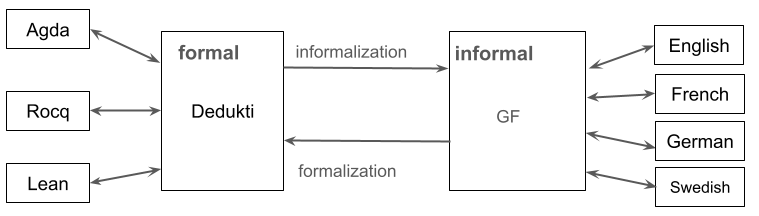
\includegraphics[width=0.82\textwidth]{simplified-informath.png}
\caption{The architecture of Informath: Dedukti as the formal interlingua, GF as the informal one.}
\label{fig:arch}
\end{figure}

Informath (Figure~\ref{fig:arch}) has two interlinguas. On the formal side, \textbf{Dedukti}
\cite{assaf-al-2023} is a minimal logical framework, the $\lambda\Pi$-calculus modulo rewriting,
designed as a hub between proof systems. Informath uses a fixed Dedukti theory of sets,
propositions and proofs:
\begin{lstlisting}
Set : Type.   Elem : Set -> Type.   Prop : Type.   Proof : Prop -> Type.
and : Prop -> Prop -> Prop.   forall : (A : Set) -> (Elem A -> Prop) -> Prop.
\end{lstlisting}
Constants beyond these base constants are user constants, such as the ones of Mathlib.

On the informal side, \textbf{GF} \cite{ranta-2004,ranta-2011} is a grammar formalism with an
\emph{abstract syntax}, a system of typed trees, and a \emph{concrete syntax} for each language,
which maps the trees to strings and back. Informath's abstract syntax has categories such as
\ttt{Prop}, \ttt{Kind}, \ttt{Exp}, \ttt{Proof}, and lexical categories such as \ttt{Noun},
\ttt{Adj}, \ttt{Fun} (``the X of Y''), \ttt{Verb2}; its concrete syntaxes are built with GF's
Resource Grammar Library (RGL) \cite{ranta-2009}, which implements inflection, agreement and
word order for some 40 languages, so that a rule such as ``$x$ is $A$'' is written once with
\ttt{mkCl} and gets the right forms in each.

The mapping between the two is defined by a \textbf{symbol table} (\ttt{.dkgf}), which assigns
to each Dedukti constant a wording, either a GF tree or an example string that the grammar
parses:
\begin{lstlisting}
Nat__minFac : "the smallest prime factor of #1" | $\operatorname{minFac}(#1)$
IsPrimePow  : "#1 is a prime power"
Eqt         : "#2 is equal to #3"     -- the type argument #1 is not shown
\end{lstlisting}
The string is parsed in a category \ttt{Example}, whose trees reveal the lexical category
(\ttt{Fun}, \ttt{Noun1}, \ttt{Adj2}, \ldots) and the order of the arguments. From the table,
a Dedukti statement is translated to a GF tree in a core language (MathCore), then rewritten by
natural language generation (NLG) rules into variants (in situ quantification, aggregation of
hypotheses, symbolic notation where it fits), which are ranked and linearized
\cite{ranta-2024}. A constant without an entry is shown symbolically, as
$\mathrm{IsUnit}(u)$.

\section{Prior work}

Readable formal mathematics has a long history. Mizar \cite{bancerek-al-2015} was designed to
look like mathematical text and produces the journal \emph{Formalized Mathematics}. Coscoy et
al.\ \cite{coscoy-al-1995} extracted texts from Coq (now Rocq) proof terms, which is close to
what we do for Lean's term proofs. Isabelle/Isar \cite{wenzel-1999} is a readable proof
language; Verbose Lean \cite{massot-2024} gives Lean a controlled natural language for
teaching, in which tactic proofs read like texts, and inspired our treatment of tactic proofs.
In the other direction, controlled natural languages such as Naproche \cite{cramer-al-2009,
koepke-2025}, ForTheL \cite{paskevich-2007} and MathNat \cite{humayoun-raffalli-2010} are
parsed into formal languages. GF has been used for mathematical language from the start
\cite{hallgren-ranta-2000,ranta-2011c,kelber-al-2025}, and GFLean \cite{pathak-2024}
autoformalizes a fragment of English into Lean with GF.

Neural approaches have used LLMs to informalize Lean, notably the Herald dataset of Mathlib
statements annotated in natural language \cite{gao-al-2025}, and to autoformalize, with
symbolically generated data as one source \cite{jiang-al-2024,huang-al-2025}. Our work is
complementary: the translation itself is symbolic, but the lexicon that it needs is inferred
from Mathlib's own text, and the system was built with an AI agent.

\section{From Lean code to natural language}
\label{sec:pipeline}

The pipeline has four steps.

\paragraph{1. Export to Dedukti.} A Lean program, \ttt{Export.lean}, imports Mathlib modules and
translates each declaration's elaborated type, and the definiens of definitions and term proofs,
to Informath's Dedukti. A binder $(x : \alpha)$ with $\alpha : \ttt{Type}$ becomes
$(x : \ttt{Elem}\ \alpha)$, one with $\alpha : \ttt{Prop}$ a hypothesis, and
$(\alpha : \ttt{Type}\ u)$ becomes $(\alpha : \ttt{Set})$. Implicit arguments are dropped
in applications, so that only the arguments a reader sees in Mathlib remain. An instance
binder \ttt{[CommMonoid M]} becomes a hypothesis \ttt{Proof (CommMonoid M)}, a class is
declared as a predicate, and a bundled function applied by coercion (\ttt{DFunLike.coe f x})
becomes a constant \ttt{f\_\_app} with its own type. A table of 39 mappings sends Lean's logic
and arithmetic (\ttt{Dvd.dvd}, \ttt{Nat.Prime}, \ttt{HAdd.hAdd}, \ttt{Iff}) to Informath's base
constants, whose wordings are part of Informath. The output is meant to be read, not checked:
dropping implicit arguments loses information a type checker would need.
For example, the Lean theorem
\begin{lstlisting}
theorem Irreducible.not_dvd_isUnit {M : Type*} [CommMonoid M] {p u : M}
    (hp : Irreducible p) (hu : IsUnit u) : ¬p ∣ u
\end{lstlisting}
is exported with its implicit variables and its instance as hypotheses, as a theorem is stated
with all of them, and its proof term with them as $\lambda$s:
\begin{lstlisting}
def Irreducible__not_dvd_isUnit : (M : Set) -> (_ : Proof (CommMonoid M)) ->
    (p : Elem M) -> (u : Elem M) -> (hp : Proof (Irreducible p)) ->
    (hu : Proof (IsUnit u)) -> Proof (not (divide p u)) :=
  M => x => p => u => hp => hu =>
    mt (divide p u) (IsUnit p)
       (ifI (divide p u) (IsUnit p) (h => isUnit_of_dvd_unit M p u h hu))
       (Irreducible__not_isUnit M p hp).
\end{lstlisting}
Here \ttt{divide} and \ttt{not} are Informath's base constants, mapped from \ttt{Dvd.dvd} and
\ttt{Not}, and \ttt{ifI} is the natural deduction rule of implication introduction.
The formula reading of the statement is
$M \in \mathrm{Set}, \mathrm{CommMonoid}(M), p, u \in M, \mathrm{Irreducible}(p),
\mathrm{IsUnit}(u) \vdash \neg (p \mid u)$; its verbal reading is shown in
Section~\ref{sec:examples}.

\paragraph{2. Readings.} RunInformath translates the Dedukti declarations with the base table,
Mathlib's table (Section~\ref{sec:tables}) and the grammar, and gives a reading in each language
and a formula in \LaTeX. The index of all 705 statements is built in one call per mode, so that
the grammar of five languages (8 MB) is loaded once. German linearization turned out to be
exponential in nested noun phrases (three levels of ``the maximum of'' took 35 seconds), so
German is read apart, with a time limit of one second per statement.

\paragraph{3. Term proofs.} A definiens that is a proof term is translated to a sequence of
proof units: each $\lambda$ becomes an assumption (``Let $n$ be an element of $\mathbb{N}$'',
``Assume that $p$ is prime''), each application of a lemma a conclusion, justified by the lemma.
Lean's logical constructors are mapped to natural deduction rules in Dedukti.

\paragraph{4. Tactic proofs.} Most of Mathlib's proofs are tactic scripts, whose text says
little: \ttt{rw [hn, mul\_one]}. Following the idea of Verbose Lean \cite{massot-2024}, we use
the goals instead. The exporter elaborates the module again with Lean's info trees, and records
for each tactic of a sequence the goal before it and the goals after it, translated to Dedukti.
A step then becomes units by comparing them: new hypotheses are assumed or stated, a closed
goal is a conclusion, a changed goal is ``it is enough to show that \ldots'', several goals are
cases. Each unit keeps the tactic as its justification:
\begin{lstlisting}
theorem Prime.eq_one_or_self_of_dvd {p : ℕ} (pp : p.Prime) (m : ℕ) (hm : m ∣ p) :
    m = 1 ∨ m = p := by
  obtain ⟨n, hn⟩ := hm
  have := pp.isUnit_or_isUnit hn
  rw [Nat.isUnit_iff, Nat.isUnit_iff] at this
  apply Or.imp_right _ this
  rintro rfl
  rw [hn, mul_one]
\end{lstlisting}
\begin{center}\footnotesize
\begin{tabular}{rll}
1. & Let $n$ be an element of $\mathbb{N}$ such that $p = m \times n$. & \ttt{obtain ⟨n, hn⟩ := hm}\\
2. & $m$ is a unit or $n$ is a unit. & \ttt{have := pp.isUnit\_or\_isUnit hn}\\
3. & $m = 1$ or $n = 1$. & \ttt{rw [Nat.isUnit\_iff, Nat.isUnit\_iff] at this}\\
4. & It is enough to show that if $n = 1$, then $m = p$. & \ttt{apply Or.imp\_right \_ this}\\
5. & Assume that $n = 1$. & \ttt{rintro rfl}\\
6. & $m = p$. & \ttt{rw [hn, mul\_one]}
\end{tabular}
\end{center}
The same units are read in the other languages: ``Stačí ukázat, že jestliže $n = 1$, pak
$m = p$'', ``Es genügt zu zeigen, dass \ldots''.

\paragraph{Outputs.} The results are shown on web pages, one per part of Mathlib, where each
declaration has its Lean source, its Dedukti translation (folded), its readings and formula,
and its proof text \cite{mathlib-informath}. A stand-alone program, \ttt{mathlib-informath},
does the same for any Lean file or code on standard input, as plain text, HTML or PDF, in about
40 seconds, most of which Lean spends loading Mathlib.

For instance, the code on standard input
\begin{lstlisting}
theorem t (n : ℕ) (h : 0 < n) : n ≠ 0 := by omega
\end{lstlisting}
gives, with \ttt{-languages=Eng,Ger},
\begin{lstlisting}
t (theorem)
  English: Let $n$ be a natural number such that $0 < n$. Then $n \neq 0$.
  German: Sei $n$ eine natürliche Zahl derart, dass $0 < n$. Dann $n \neq 0$.
  Proof, English:
    1. $n \neq 0$.   [omega]
\end{lstlisting}
A user's own symbol table can be added on top of Mathlib's, for the concepts that the code
defines itself.

\section{Inferring the symbol tables}
\label{sec:tables}

Informath's own lexicon covers basic mathematics; Mathlib has tens of thousands of concepts.
The first tables were written by hand: 108 entries for the constants that our first modules use,
with suggestions from docstrings and names checked by the grammar. This does not scale, so we
infer a table for all of Mathlib's definitions.

\paragraph{The definitions.} \ttt{export --definitions} imports all of Mathlib (20 seconds) and
exports every declaration that may need a wording: definitions, structures, classes, fields,
inductive types, but not theorems, instances, tactics, notations, auxiliary or deprecated
declarations. Of 56,852 such constants, 38,667 remain after filtering, each with its Dedukti
type, explicit argument names and docstring. Its type tells its category: a function or constant
(\ttt{Exp}), a type (\ttt{Kind}), or a predicate (\ttt{Prop}).

\paragraph{Candidates.} For each definition, candidate wordings are made in two ways.
\emph{From the docstring}, patterns pick noun phrases and predicates: ``\ttt{`f n`} is the X of
\ttt{`n`}'', ``The X of \ldots\ is'', ``A set is X if'', with the backticked argument names
replaced by their positions \ttt{\#1}, \ttt{\#2}. \emph{From the name}, the last component is
split at capitals and underscores, and Mathlib's abbreviations are spelled out (\ttt{minFac}:
minimum factor; \ttt{card}: cardinality; \ttt{AddMonoidHom}: additive monoid homomorphism,
with \emph{Add} as a modifier rather than ``sum''). The name gives ``the X of \ttt{\#1}'' for a
function, ``X of \ttt{\#1}'' for a type, ``\ttt{\#1} is (a) X'' for a predicate
(\ttt{IsCountablyCompact}: ``\ttt{\#1} is countably compact''), ``\ttt{\#1} has X'' for one
named after a verb (\ttt{HasLimits}, \ttt{PreservesFiniteLimits}). A few conventions needed
special rules: a constructor \ttt{Bicone.ofLimitCone} is named after its namespace (``the bicone
of \ttt{\#1}''), a function \ttt{pointOfClosedPoint} after its head, but a type
\ttt{PartitionOfUnity} keeps its ``of''.

For example, \ttt{Ordinal.cof : Ordinal → Cardinal} has the docstring ``The cofinality on an
ordinal is the \ttt{Order.cof} of any isomorphic linear order''. Its first pattern gives
``the cofinality on an ordinal of \ttt{\#1}'', which does not parse; with the generic
prepositional phrase cut out, ``the cofinality of \ttt{\#1}'' does, and it is also what the name
gives, as \ttt{cof} is spelled out as \emph{cofinality}. Since the candidate shares a word with
the name, it is accepted; a docstring wording that shares no word with the name, such as ``the
ring'' for \ttt{HahnSeries.toPowerSeries}, is not tried.

\paragraph{Checking.} All 41,000 candidates are parsed by the grammar in one call (30 seconds).
A candidate is accepted if its parse has the category and the arity of the constant; the first
one accepted becomes the entry. Many constants take explicit parameters before their main
arguments (a category, a Grothendieck topology); a wording may leave them out, as \ttt{Eqt}
above leaves out the type. But leaving out the wrong argument gives a false reading:
\ttt{IsRelUpperSet s P} was first read ``$P$ is a relation upper set''. A predicate of two
objects is therefore read as binary, ``\ttt{\#1} is a relative upper set with respect to
\ttt{\#2}'', with the subject chosen by the docstring (the argument that it does \emph{not} name
after ``relative to'', ``for'', ``over''), and without such a clue it gets no reading. We prefer
a symbolic reading to a wrong one.

\paragraph{The lexicon.} Candidates fail mostly because of unknown words. These are added to the
grammar: a word that recurs in the candidates gets a noun, adjective, adverb or verb entry, with
its category and plural from the RGL's English dictionary (\ttt{DictEng}), and a word that the
dictionary lacks is admitted if three docstrings use it. Junk had to be filtered out by hand-made
lists: docstrings contain function words that the dictionary lacks (\emph{because},
\emph{without}) and Lean jargon (\emph{simproc}, \emph{defeq}). The result is 507 English words,
from \emph{cocone}, \emph{equicontinuous} and \emph{hypercover} to \emph{Zariski}.

For the other languages, we first tried GF's WordNet \cite{miller-1995,angelov-2020}, choosing
senses by their domain tags: only 117 of 789 words were found, 13 of them in a sense tagged
\emph{mathematics}, and even those were mixed (\emph{hexagon}: \emph{Sechseck}, correct;
\emph{minus}: \emph{Weg}, wrong; \emph{triplet}: \emph{trois}, wrong). Mathlib's jargon is not
there. We therefore keep the translations in a table, one line per word with its French,
German, Swedish and Czech forms (gender, plural), written by Claude and to be reviewed, with an
empty cell where unsure; the grammar modules are generated from it. Where a language lacks a
word, the index keeps the reading made without the generated table, which shows the constant
symbolically.

\paragraph{The lexicon, a second time.} Most definitions left without an entry have a word in
their name that the grammar lacks as a noun or adjective, although its lexicon (4,560 words) has
a word for it. A second round replaces such words: a verb by its nominalization, after its object
(\ttt{restrictScalars}: ``the scalar restriction of \ttt{\#1}''); an abbreviation by the word of
the lexicon that it abbreviates and that the docstrings of the definitions named with it use
most (\ttt{denom}: denominator, \ttt{coeq}: coequalizer); a proper name by its spelling
(\ttt{kronecker}: Kronecker); and \ttt{desc} and \ttt{forget} by ``the induced morphism'' and
``the forgetful functor''. As long names read word by word were mostly wrong, the round is
restricted to names of at most two words. It gives 887 entries with 135 replacements, which are
listed for review.

\section{Who contributed what}
\label{sec:who}

Table~\ref{tab:sources} shows where the wordings of the definitions come from: most from names,
an eighth from docstrings, 887 from names with words of the lexicon, and a few from the
hand-written table, which overrides the
generated one. Table~\ref{tab:who} divides the work between the existing Informath, the first
author's prompts and decisions, and the AI agent.

\begin{table}[t]
\centering\footnotesize
\begin{tabular}{lrrrr}
\toprule
& functions, constants & types & predicates & all \\
\midrule
definitions & 31,858 & 2,464 & 4,345 & 38,667 \\
with a wording & 23,059 & 1,816 & 1,866 & \textbf{26,741} (69\%) \\
\midrule
\multicolumn{4}{l}{read in English (Section~\ref{sec:allread}): with a reading} & \textbf{38,424} (99\%) \\
\multicolumn{4}{l}{\quad with no constant shown symbolically} & about 12,200 (32\%) \\
\multicolumn{4}{l}{read as a formula} & \textbf{38,460} (99\%) \\
\multicolumn{4}{l}{read in French: with a reading} & \textbf{38,064} (98\%) \\
\multicolumn{4}{l}{\quad with no constant shown symbolically} & about 12,000 (31\%) \\
\midrule
\multicolumn{5}{l}{the wordings from: names 22,304; docstrings 3,488; names with the lexicon 887;
the hand-written table 62} \\
\bottomrule
\end{tabular}
\caption{The symbol table of Mathlib's definitions.}
\label{tab:sources}
\end{table}

\begin{table}[t]
\centering\footnotesize
\begin{tabular}{p{0.3\textwidth}p{0.3\textwidth}p{0.32\textwidth}}
\toprule
\textbf{Already in Informath} & \textbf{From the first author} & \textbf{By Claude} \\
\midrule
The GF grammar and its concrete syntaxes on the RGL; the Dedukti theory; symbol tables with
verbal, symbolic and macro forms; NLG with variants and ranking; proof texts from terms &
The goal; the choice of Mathlib's prime numbers as the first case; the contents of the pages;
loading the grammar once; the idea of tactic proofs as proof units; the time limit for German;
WordNet as a resource; a reviewable table rather than generated code; the stand-alone program &
\ttt{Export.lean} with its translation rules; the index and the pages; the table inference, the lexicon generation and the second round with the lexicon; the translations table; the Informath extensions this needed
(multilingual proof texts, \ttt{-tactic-proof}, aggregated hypotheses, Czech and Swedish
modules) \\
\bottomrule
\end{tabular}
\caption{The division of labour.}
\label{tab:who}
\end{table}

Some of the decisive steps were the human's: the diagnosis of a parameter explosion in the GF
compiler (a list category whose concrete functions grew to $5 \times 10^{13}$), the reason why
size-optimized grammars broke all proof texts (the proof units were not reachable from the start
category), and the decision to keep the translations reviewable. Others were the agent's:
the iteration over hundreds of failing cases, measuring each change on the whole of Mathlib, and
testing a resource (WordNet) before relying on it. All the words written by Claude, in all
languages, are to be reviewed by native speakers.

\section{Examples}
\label{sec:examples}

\paragraph{Definitions.} Mathlib defines a prime number as an irreducible element:
\begin{lstlisting}
def Prime (p : ℕ) := Irreducible p
\end{lstlisting}
\reading{Let $p$ be a natural number. Then $p$ is prime, if $p$ is irreducible.\\
Soit $p$ un nombre naturel. Alors $p$ est premier si $p$ est irréductible.\\
Låt $p$ vara ett naturligt tal. Då är $p$ primt, om $p$ är irreducibelt.}
\noindent Wordings from the generated table, with the arguments shown by their names:
``the cofinality of $o$'', ``the normalizer of $H$'', ``$C$ has limits'', ``$F$ preserves
finite limits'', ``$P$ is separated with respect to $J$'', ``$M$ is a perfect matching''.

\paragraph{Theorems.} Euclid's theorem in five languages:
\begin{lstlisting}
theorem exists_infinite_primes (n : ℕ) : ∃ p, n ≤ p ∧ Prime p
\end{lstlisting}
\reading{Let $n$ be a natural number. Then there exists a natural number $p$, such that
$n \leq p$ and $p$ is prime.\\
Soit $n$ un nombre naturel. Alors il existe un nombre naturel $p$ tel que $n \leq p$ et $p$ soit
premier.\\
Sei $n$ eine natürliche Zahl. Dann gibt es eine natürliche Zahl $p$, derart, dass $n \leq p$
und $p$ prim ist.\\
Låt $n$ vara ett naturligt tal. Då finns det ett naturligt tal $p$, så att $n \leq p$ och $p$
är primt.\\
Nechť $n$ je přirozené číslo. Tedy existuje přirozené číslo $p$, \textcolor{red}{takový}, že
$n \leq p$ a $p$ je prvočíselné.}
\noindent The aggregation of hypotheses makes statements with many variables readable:
\reading{Let $M$ be a set such that $M$ is a commutative monoid. Let $p$ and $u$ be elements of
$M$ such that $p$ is irreducible and $u$ is a unit. Then $p$ does not divide $u$.}
\noindent (\ttt{Irreducible.not\_dvd\_isUnit}; the Lean statement has the implicit \ttt{M},
\ttt{p}, \ttt{u} and the instance \ttt{[CommMonoid M]}.)

\paragraph{Term proofs.} The definiens of \ttt{exists\_infinite\_primes}, with its local
definitions and \ttt{have}s, becomes a proof text of twelve lines, which starts:
\reading{1. Let $n$ be an element of $\mathbb{N}$.\quad 2. $0 < n!$.\quad 3. The successor of
$0$ is less than the successor of $n!$.\quad 4. $n! + 1 \neq 1$.\quad 5.
$\mathrm{minFac}(n! + 1)$ is prime.\quad \ldots}
\noindent Each line is justified by the lemma it applies (\ttt{Nat.factorial\_pos},
\ttt{Nat.succ\_lt\_succ}, \ldots), linked to its own entry.

\paragraph{Bad cases.} Not everything reads well:
\begin{itemize}
\item a constant without a wording stays symbolic: ``Let $n$ be a natural number such that
  $\mathrm{Coprime}(2, n)$'' in French, where the English has ``$2$ and $n$ are coprime'';
\item mismatched agreement: Czech \emph{takový} above, which should be \emph{takové}; ``Let
  $s$ be \textcolor{red}{a} upper set'';
\item literal wordings: Swedish ``lika \textcolor{red}{till}'' for ``equal to'' (\emph{lika
  med}), as the table's ``is equal to'' is parsed word by word;
\item generated wordings that say little: \ttt{BoundedOrderHom.dual}, a bundled map without
  explicit arguments, is ``the dual'';
\item German: ``Dann $2 \leq p$'' without a verb, and 51 statements over the time limit.
\end{itemize}

\section{Results}

Table~\ref{tab:results} shows the readings of 705 statements from 19 modules: Mathlib's order
and lattice definitions, the algebra that the prime numbers import, the prime numbers, and
prime factorizations. A statement is \emph{fully worded} if no Lean constant in it is shown
symbolically. Every statement has a formula, and 264 declarations come with their definiens.
Of the 242 term proofs, 240 have a proof text in each language; of the 242 tactic proofs, the 25
of \ttt{Nat.Prime.Defs} have one so far, in five languages. In 26 statements a language keeps
the older, more symbolic reading because it lacks a generated word. The whole index takes about
ten minutes on a laptop, most of it for German.

\begin{table}[t]
\centering\small
\begin{tabular}{lrrrrrr}
\toprule
& statements & English & French & Czech & German & Swedish \\
\midrule
Order, lattices & 354 & 291 & 289 & 289 & 248 & 289 \\
Algebra & 29 & 29 & 29 & 29 & 28 & 28 \\
Prime numbers & 128 & 125 & 125 & 125 & 125 & 125 \\
Factorizations & 194 & 143 & 143 & 143 & 132 & 142 \\
\midrule
all & 705 & \textbf{588} & \textbf{586} & \textbf{586} & \textbf{533} & \textbf{584} \\
\bottomrule
\end{tabular}
\caption{Fully worded statements, by language.}
\label{tab:results}
\end{table}

For all of Mathlib, the generated table gives 69\% of the definitions a wording
(Table~\ref{tab:sources}), checked by the grammar for category and arity but not reviewed by
hand. Random samples during the development showed classes of errors, which led to the rules
of Section~\ref{sec:tables}.

\paragraph{A sample.} To estimate the quality of the final table, Claude judged a random sample
of 60 generated wordings against the definitions' docstrings (Table~\ref{tab:sample}): a wording
is \emph{good} if it says what the definition is in idiomatic terms, \emph{acceptable} if it is
vague but not wrong, and \emph{wrong} if it says something else or nothing. This is the judgement
of one annotator, the second author, and is not yet reviewed.

\begin{table}[t]
\centering\small
\begin{tabular}{lp{0.56\textwidth}r}
\toprule
& examples & \\
\midrule
good & ``$C$ has injective resolutions'', ``$f$ is differentiable'', ``the wide pullback of $s$'',
       ``the Grothendieck topology of $T$'', ``the smallest prime factor of $x$'' & 22 \\
acceptable & ``the evaluation of $g$ and $p$'' (\ttt{MvPolynomial.eval\textsubscript{2}}), ``the
       adjunction'', ``the tail of $p$ and $\mathit{len\_pos}$'' (a proof argument shown) & 20 \\
wrong & ``the vector multiplicative vector of $w$ and $v$'' (\ttt{vecMulVec}), ``the unit
       product of $u$ and $w$'' (\ttt{unitsSMul}), ``the opposite opposite of $S$''
       (\ttt{opUnop}), ``$R$ is a continuous square root'' (a class saying that one exists) & 18 \\
\bottomrule
\end{tabular}
\caption{A random sample of 60 generated wordings, judged by the second author.}
\label{tab:sample}
\end{table}

Two thirds are thus usable, and the predicates fare best: of the eleven in the sample, nine are
good. The wrong ones are mostly composite names read word by word
(\ttt{presheaf\-Hom\-Sections\-Equiv}: ``the presheaf homomorphism section equivalence''), and
abbreviations spelled out wrongly in context (\emph{SMul} is a scalar multiplication, not a
product). Proof arguments and unnamed arguments ($\#4$) should not be shown, and
\ttt{LibraryNote}, documentation without mathematical content, should have been filtered out.

\paragraph{A sample of the second round.} 60 of the 887 entries made with the lexicon, judged in
the same way, are 40 good, 14 acceptable and 6 wrong (10\%, against 30\%): ``the scalar
restriction of $f$'' and ``$f$ is differentiable on $s$'' are good; ``the composition application
of $c$ and $i$'' (\ttt{applyComposition}) and ``the finite extension of $K$ and $L$''
(\ttt{finiteExts}, a set of extensions) are wrong.

\paragraph{All the definitions in English.}
\label{sec:allread}
Finally, all 38,667 definitions were read in English and as formulas, and then in French, as the statements on the
pages are: each definition's statement, with its definiens where it has one (25,491 of the
exported constants have one that the exporter translates), by the full symbol table. With eight
RunInformath processes and a time limit of one second per definition and mode, this took about
half an hour on a laptop. 38,424 definitions (99\%) got a reading, 217 went over the time
limit, and 26 got none; 38,460 got a formula. About 12,200 readings (32\%) show no constant
symbolically; the others show the constants that
have no wording, often from the definiens, as operators. The readings are published on 111
static pages of at most 400 definitions, by part of Mathlib, with a search page over all of
them. For example, \ttt{Quiver.IsThin}:
\reading{Let $V$ be a set. Then $V$ is thin, if for all elements $a$ and $b$ of $V$, the set of
homomorphisms of $a$ and $b$ is a subsingleton.\\[1mm]
$V \in \mathrm{Set} \vdash \operatorname{IsThin}(V) :\Leftrightarrow \forall a \in V .\ \forall b \in V .\
\mathrm{Subsingleton}(\operatorname{Hom}(a, b))$}
\noindent French uses the same pipeline and symbol table, as Informath parses the English
wordings into GF trees and linearizes them in French; the French rows are hidden on the pages
until asked for, as on the other pages. The French reading of \ttt{Quiver.IsThin} is
\reading{Soit $V$ un ensemble. Alors $V$ est fin si pour tous les éléments $a$ et $b$ de $V$,
l'ensemble d'homomorphismes de $a$ et $b$ est un sous-singleton.}
\noindent where \emph{fin} for \emph{thin} is a word to be reviewed. In the first run, 9,774 of the
French readings (26\%) used a word that had no French form: 263 words of Informath's lexicon,
from its parts that were written for English only (the Godement, HoTT and Naproche lexicons),
led by \emph{opposite} (in 1,554 readings), \emph{lift} (1,053) and \emph{carrier} (950).
Claude wrote their French forms (\emph{opposé}, \emph{relèvement}, \emph{ensemble sous-jacent}),
to be reviewed, and the affected definitions were read again: 38,064 definitions (98\%) now
have a French reading, and 12,043 of them show no constant symbolically, almost as many as in
English (12,155).
4 readings still use a word without a French form, which the pages show in English, marked. The
other three languages can be read in the same way.

\section{Known problems and open issues}
\label{sec:problems}

\paragraph{Coverage.} All of Mathlib's definitions are read, but only in English, as formulas
and in French, and its
theorems only in part: the 705 statements of the pages are a small part of its 194,000 theorems,
which the same pipeline could read, with their proofs, but which we have not run on. Of the
definitions, 217 go over the time limit, and two thirds of the readings still show some constant
symbolically, mostly constants of the definientia that have no wording. The generated table is
unreviewed, and in our samples 18 of 60 of its first wordings (30\%) and 6 of 60 of those made with
the lexicon (10\%) are wrong: composite names
(\ttt{quotientIdealMapEquivTensorQuot}) become nonsense when read word by word; bundled maps
without arguments get bare readings; about 2,500 unknown words are abbreviations of jargon that
we do not spell out. Most tactic proofs have no text yet, and long \ttt{simp} goals make poor
reading.

\paragraph{Language.} Agreement of ``such that'' with an existential's kind fails in Czech and
French; multi-letter variables (\ttt{self}, \ttt{motive}) are shown as constants; a lemma used
unapplied in a proof term gives garbled text; the meaning of $\leq$ on finite sets is
``subset'', which the reading does not know. The French words added for the definitions and the
French readings themselves are not checked. The words of four languages need native review,
and German linearization needs a fix in the RGL.

\paragraph{Correctness.} The translation is compositional, but the exporter drops implicit
arguments, so the Dedukti code is not type-checked; a reading is as correct as the table entries
it uses, and the generated entries are checked only by the grammar. A back-translation from the
readings to Dedukti and a type check would close this loop, as Informath supports in the other
direction.

\section{Conclusion}

Symbolic informalization of Lean is feasible at the scale of Mathlib if the lexicon can be
inferred: Mathlib's naming conventions and docstrings, with the grammar's own lexicon, give wordings to 69\% of its
definitions, and a grammar can check them. With them, all of Mathlib's definitions have been
read in English, as formulas and in French, a third of them with no symbolic residue in
English, in an hour on a laptop. The readings are faithful by construction, and they
come in five languages at once. What the method does not give is judgement: which wording is
right, which word a language uses, when a reading is false although it parses. That remained
the human's part, in a collaboration where the AI agent did most of the construction and the
measuring.

\paragraph{Acknowledgements.} The first author thanks Krasimir Angelov for the RGL work on Czech
and German that this project relied on, and Josef Urban for introducing him to agentive coding.
This work has been supported by the European Research Council through the grants
\textit{NextReason} (Grant ID 101200949) and \textit{MALINCA} (Grant ID 101167526).

\bibliographystyle{plain}
\bibliography{resources/gf-bib,paper}

\end{document}
